PocketShelf is an inventory IOS/Android application. Our application consist of many features among which adding item/shelf, search item for each user with Augmented reality experience is the key feature of our application. Diagram below show the overall high level feature of our application.


\begin{figure}[h!]
	\centering
 	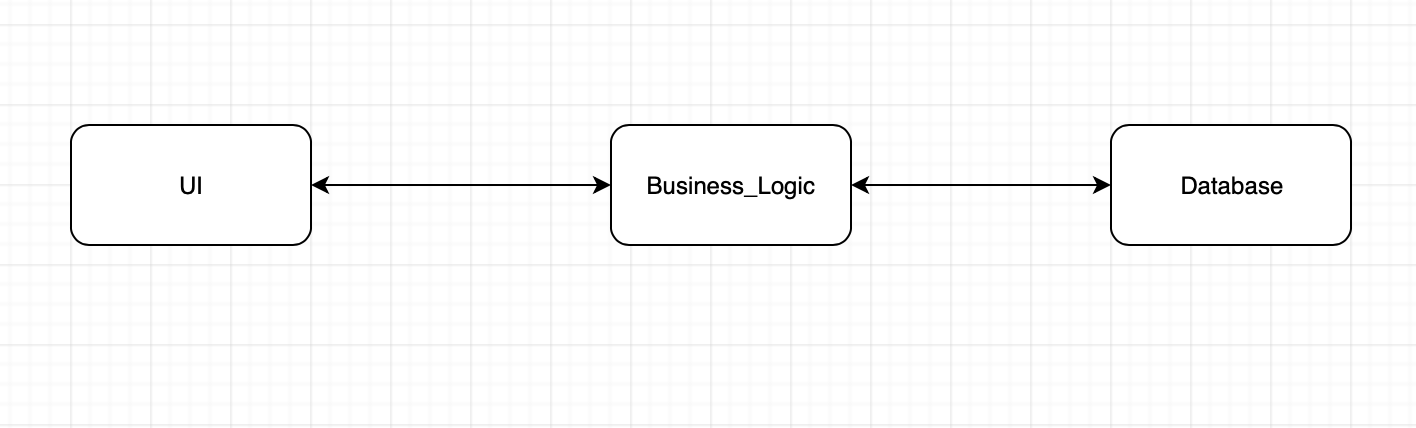
\includegraphics[width=0.90\textwidth]{images/overview}
 \caption{A simple architectural layer diagram}
\end{figure}

\subsection{UI}
UI is the graphic feature of the application mainly responsible for the displaying information and interact with the user. UI consist of login subsystem responsible for taking userid and password from user. Registration subsystem is responsible to take userid, email, password, full name from the user. Add\_Shelf subsystem is responsible for taking the shelf description from the user. Add\_Item is responsible for taking item description from user. Search subsystem is responsible for taking user input via QR code or input text. After any kind input and options chosen by the user UI\_Controller will send all user input and the option chosen by the user to Business\_Controller in Business\_Logic. UI\_Controller also accept the input messages from the Business\_Controller, stating successful completion of the chosen task by the user.

\subsection{Business\_Logic}
Business\_Logic is the logical controller for the application. It is responsible for taking input fro UI\_Controller, work accordingly based on the input given by UI\_Controller and work with DB\_Controller. If the UI\_Controller get any kind of input from user it validate it in order to prevent SQL injections and prevent all sort of the invalid input that can be given by the user before sending it to DB\_Controller. If UI\_Controller sends the item description to add to the shelf, it will create QR for the entry, append it with the description and forward it to DB\_Controller to save it to Database. If UI\_Controller sends any item information to search from database, Business\_Logic will validate the input and the sends the item description to the DB\_Controller, once item is retrieve and received by Business\_Logic it fetch the image associated to the item and sends that image to UI\_Controller which is shown to the user.


\subsection{Database}
Database the is core functioning elements of our application, which will handles every thing relate to the database. DB\_Controller will accepts input from the Business\_Controller and work according to that. DB\_Controller also return the Boolean value to the Business\_Controller to indicate successful or unsuccessful completion of the queries. Along with the item needed if asked by Business\_Controller. Login\_mgt will checks the user input against the input in the database, if no result found it return false. Reg\_mgt will add the new user to the database. Shelf\_mgt will add item to the database along with the available shelf. Once added DB\_Controller will return true with the shelf description to the Business\_Controller. Search\_mgt will take input from Business\_Controller, then it will look up in the database, if found it will return the item  the Business\_Controller.   